\section{Reducing Task Error}
\label{sec:reducing_error}

\begin{figure}[t]
    \centering
    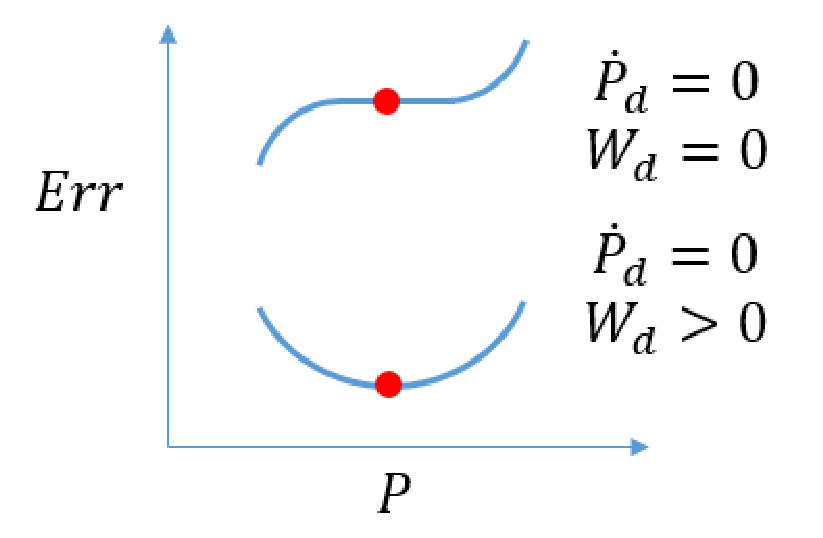
\includegraphics[width=1.8in]{error_graphs_modified}
    \caption{Top Line: moving the point does not change the error, thus the desired movement is zero, however, it is not important to achieve zero movement, thus $\Pinvweight_d = 0$.  Bottom Line: error is at a local minimum; thus moving the point increases error.}
    \label{fig:error_examples}
\end{figure}

\begin{algorithm}[t]
\caption{CalculateCorrespondences$(\deformconfig, \target)$}
\begin{algorithmic}[1]
    \State $\correspondences = [ \emptyset ]_{1 \times \ndeformpoints}$
    \For {$\targetidx \in \{ 1, 2, \dots, \ntargetpoints \}$}
        \State $\deformidx \gets \argmin_{j \in \{ 1, 2, \dots, \ndeformpoints \}} d_\textrm{Dijkstras}(\targetK, \deformconfigJ)$
        \State $d \gets d_\textrm{Dijkstras}(\targetK, \deformconfigI)$
        \State $\correspondences[\deformidx] \gets \{ \correspondences[\deformidx] \cup (\targetidx, d)\}$
    \EndFor
    \State \Return $\correspondences$
\end{algorithmic}
\label{alg:calculate_correspondences}
\end{algorithm}

\begin{algorithm}[t]
\caption{FollowNavigationFunction$(\deformconfig, \correspondences)$}
\begin{algorithmic}[1]
    \State $\deformvel_e \gets \zero_{\deformCspacesize \times 1}$
    \State $\Pinvweight_e \gets \zero_{\ndeformpoints \times 1}$
    \For {$\deformidx \in \{ 1, 2, \dots, \ndeformpoints \}$}
        \For {$(\targetidx, d) \in \correspondences[\deformidx]$}
            \State $\deformvelIpre{e} \gets \deformvelIpre{e} +$ DijkstrasNextStep$(\deformconfigI, \targetidx)$ \label{alg:follow_nav:accumulate}
            \State $\PinvweightIpre{e} \gets \max(\PinvweightIpre{e}, d)$ \label{alg:follow_nav:max}
        \EndFor
    \EndFor
    \State \Return $\deformvel_e, \Pinvweight_e$
\end{algorithmic}
\label{alg:follow_nav_function}
\end{algorithm}

We build on previous work~\cite{Berenson2013}, splitting the desired deformable object movement into two parts: an error correction part and a stretching correction part. When defining the direction we want to move the deformable object to minimize error we calculate two values; which direction to move the deformable object points $\deformvel_e$ and the importance of moving each deformable object point $\Pinvweight_e$. This is analogous to computing the gradient of error, as well as an ``importance factor'' for each part of the gradient. We need these weights to be able to differentiate between points of the object where the error function is a plateau versus points where the error function is at a local minimum~(Fig.~\ref{fig:error_examples}). Typically this is achieved using a Hessian, however our error function does not have a second derivative at many points. 

In order to calculate $\deformvel_e$ and $\Pinvweight_e$, we start by defining a workspace navigation for each target point $\targetK \in \target$ towards $\targetK$ using Dijkstra's algorithm. This gives us the shortest collision-free path between any point in the workspace and the target point, as well as the distance travelled along that path. Using these distances, at every timestep we for every target point $\targetK$, we recalculate which point on the deformable object $\deformconfigI$ is closest (Alg.~\ref{alg:calculate_correspondences}). The directions each navigation function indicates are added together to define the overall direction to manipulate a point (Alg.~\ref{alg:follow_nav_function} line \ref{alg:follow_nav:accumulate}). For the importance factors $\Pinvweight_{e,\deformidx}$, we take only the largest distance that $\deformconfigI$ would have to move as a way to mitigate discretization effects (Alg.~\ref{alg:follow_nav_function} line \ref{alg:follow_nav:max}).